\section{Scikit-learn - Class Imbalance}
\label{subsection:scikit-class-imbalance}

In this section, similar to NLTK, the class imbalance issue is tackled and will use the same under sampling of the majority class, over sampling of the minority class and hybrid sampling techniques that were initially explored in Section \ref{subsection:nltk-class_imbalance}.

However, before addressing the class imbalance, two other very useful features of Scikit-Learn, the pipeline and grid based searches, are utilised to fine turn the classifiers from the previous section.

\subsection{Pipeline and Grid Search}

The Scikit-Learn \verb|Pipeline| class, when used in conjunction with the \verb|GridSearchCV| class, can be used to assemble several transformation and estimator steps that can be executed together in sequence while setting different parameters for each transformer or estimator. In this tentative examining of these features the transformer that will be examined is the TF-IDF transformer and the estimators, or classifier, will be the Multinomial Naive Bayes. Later, when looking at cost based estimation, the Linear Support Vector classifier will also be examined. 

When using a grid search, an initial range of values for a set of parameters are defined that are then exhaustively examined such that all possible combinations of parameter values are tested. Where parameters are numeric the initial range of values are typically well spread out and then fine tuned over a number of searches until the optimal value is found. When applied to the Multinomial Naive Bayes estimator with the TF-IDF transformer, the initial parameter ranges applied were as shown in Listing \ref{lst:chapter5.4:snipet_01}. The data is then fitted and the best score achieved that can be obtained, as well as the parameter values that yielded the best score, are returned. Some knowledge of the transformers and estimator used in the grid search is assumed as blindly setting arbitrary values for random parameters could give unexpected results that on the surface appear good but on closer examination do not yield the desired results. When used with the Multinomial Naive Bayes estimator the default scoring value is the overall accuracy of the model. The scoring value could be set to score on recall or precision, but this could return a perfect recall score where all samples are given the same class. This would not be the desired result.

\begin{lstlisting}[caption={Using grid search to fine tune parameter values}, label=lst:chapter5.4:snipet_01]
# Create a pipeline with a transformer and a estimator
pipeline = Pipeline([
    ('tfidf', TfidfVectorizer()),
    ('clf',   MultinomialNB()),
])

# Define the parameter ranges
parameters = {
    'tfidf__stop_words': [None, 'english'],
    'tfidf__ngram_range': [(1, 1),
                           (1, 2),
                           (1, 3),
                           (2, 2),
                           (2, 3),
                           (3, 3)],
    'tfidf__norm': ['l1', 'l2'],
    'clf__alpha': [10, 1.0, 0.1, 0.01],
}
\end{lstlisting}

The results returned from the first running of the grid search object were:

\begin{spverbatim}
Done in 163.616s
Best score: 0.873
Best Parameters:
    clf__alpha:         0.1
    tfidf__ngram_range: (1, 3)
    tfidf__norm:        'l2'
    tfidf__stop_words:  None
\end{spverbatim}
 
Although further fine tuning of the \verb|alpha| parameter was performed, no further gains were made. When these parameter values were fed back into the Scikit-Learn Python script as it existed at the end of the previous section it can be seen, as shown in Figure \ref{fig:scikit_process_chart_03} and Table \ref{tab:chapter5:grid_search_01}, that whilst the overall accuracy of the model has indeed improved, this improvement was mostly achieved by a significant improvement in the precision of the positive class at the cost of a small reduction in the positive class recall. It could be argued, depending on the final production use of the model, that this reduction in positive class recall is an acceptable sacrifice given that the maximum model accuracy has been achieved. Balancing this trade off between gains in one area over losses in another will, in the final model, be determined by whether it is more important to correctly predict the most amount of bullying samples as bullying, a high recall value, while accepting that a significant proportion of not bullying sample will incorrectly be classified as bullying or is it better to maximise the precision of each class.

In Figure \ref{fig:scikit_process_chart_03} and Table \ref{tab:chapter5:grid_search_01} \verb|run_01| represents the previous manually tuned parameters and \verb|run_02| the results obtained using the parameters from the grid search.

\begin{figure}[htbp]
	\centering
	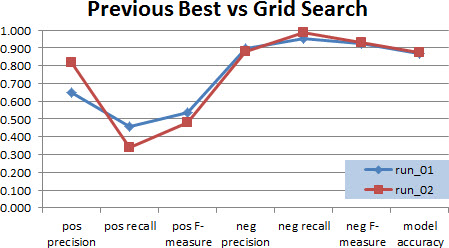
\includegraphics[width=0.6\textwidth]{Figures/Chapter5/scikit_process_chart_03.jpg}
	\caption[Scikit-Learn comparing best manual results with grid search results]{Graph showing a comparison of the results from the best manually tuned parameters against the best grid search parameters for a Multinomial Naive Bayes classifier}
	\label{fig:scikit_process_chart_03}
\end{figure}

\begin{table}[h]
	\centering
	\caption[Grid search performance and confusion matrix comparison]{Table showing a comparison of the results from best manually tuned parameters against the best grid search parameters for a Multinomial Naive Bayes classifier}
	\label{tab:chapter5:grid_search_01}
	\begin{tabular}{lrr}
		\toprule
		\textbf{Performance}& \textbf{run\_01}  & \textbf{run\_02}   \\
		\midrule
		pos precision & 0.648 & 0.816  \\
		pos recall & 0.456 & 0.342  \\
		pos F-measure & 0.534 & 0.480  \\
		neg precision & 0.898 & 0.882  \\
		neg recall & 0.950 & 0.984  \\
		neg F-measure & 0.922 & 0.930  \\
		model accuracy & 0.868 & 0.875  \\
		run time & 2.370 & 3.519  \\
		\midrule
		\textbf{Confusion} &  &   \\
		\textbf{Martix} & \textbf{run\_01} & \textbf{run\_02}  \\
		\midrule
		pos samples & 344 & 345  \\
		neg samples & 1565 & 1564  \\
		Pred Pos True Pos & 157 & 117  \\
		Pred Pos True Neg & 77 & 21  \\
		Pred Neg True Neg & 1488 & 1543  \\
		Pred Neg True Pos & 187 & 228  \\		
		\bottomrule
    \end{tabular}
\end{table}

From this point on, as class imbalance options are investigated, the pipeline and grid search classes will continue to be used. The approach is to run the pipeline grid search on the various datasets and then use the parameters returned to get the complete set of performance measures from the model.

A sample Python grid search script is given in Appendix \ref{app:grid_scikit}.

\subsection{Class Sampling}
In this section, the sampling logic previously used with the NLTK models are now applied to the pipeline grid search using Scikit-Learn Multinomial Naive Bayes and Linear Support Vector classifiers with a TF-IDF transformer. Datasets with ratios of 3:1, 2:1 and 1:1, are generated for under sampling of the majority class and over sampling of the minority class and for the hybrid approach the negative class and positive class are sampled to ratios of 70:30, 60:40 and 50:50 respectively. The results from these model executions are shown in Figure \ref{fig:scikit_process_chart_04}. 

\begin{figure}[htbp]
	\centering
	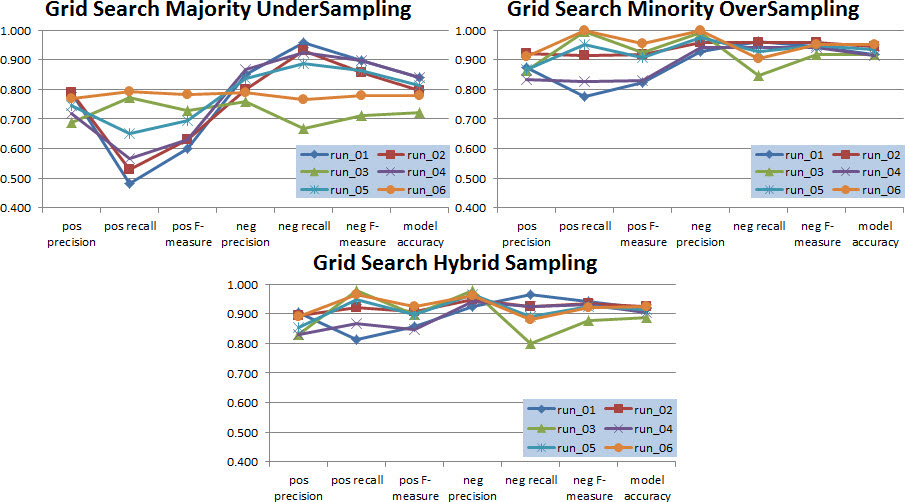
\includegraphics[width=1.0\textwidth]{Figures/Chapter5/scikit_process_chart_04.jpg}
	\caption[Scikit-Learn sampling with grid search results]{Graphs showing the performance results for grid searches using under, over and hybrid sampling with Multinomial Naive Bayes and Linear Support Vector classifiers}
	\label{fig:scikit_process_chart_04}
\end{figure}

In Figure \ref{fig:scikit_process_chart_04} \verb|run_01, 02 & 03| are the results from the Multinomial Naive Bayes classifier and reflect ratios \verb|3:1, 2:1 1:1 or 70:30, 60:40 & 50:50| respectively while \verb|run_04, 05 & 06| are the results from the Linear Support Vector classifier and are representative of the same sample ratios. With just a cursory look at these charts, it is quite clear that over sampling of the minority class and hybrid sampling both significantly out perform under sampling of the majority class. Because of these results, under sampling will not be analysed further. The actual performance values achieved for over sampling and hybrid sampling are given in Table \ref{tab:chapter5:grid_search_performance_comparison}.


\begin{table}[h]
\centering
\caption[Performance comparison of over sampling and hybrid sampling]{Table comparing the grid search performance of over sampling and hybrid sampling using Multinomial Naive Bayes and Linear Support Vector classifiers}
\label{tab:chapter5:grid_search_performance_comparison}

\begin{tabular}{rccccccc}
	\toprule
	\multicolumn{4}{c}{\textbf{Over Sampling}} \\
	\cmidrule(r){1-4}
	 & \textbf{run\_01} & \textbf{run\_02} & \textbf{run\_03} & \textbf{run\_04} & \textbf{run\_05} & \textbf{run\_06} \\
	\midrule
	pos precision & 0.874 & 0.920 & 0.864 & 0.832 & 0.868 & 0.912 \\
	pos recall & 0.776 & 0.914 & 0.994 & 0.826 & 0.952 & 1.000 \\
	pos F-measure & 0.822 & 0.916 & 0.926 & 0.830 & 0.908 & 0.954 \\
	neg precision & 0.928 & 0.958 & 0.992 & 0.942 & 0.974 & 1.000 \\
	neg recall & 0.962 & 0.958 & 0.846 & 0.942 & 0.928 & 0.904 \\
	neg F-measure & 0.944 & 0.958 & 0.916 & 0.942 & 0.948 & 0.950 \\
	model accuracy & 0.916 & 0.945 & 0.919 & 0.915 & 0.935 & 0.952 \\
	run time & 4.056 & 4.765 & 6.871 & 5.274 & 6.312 & 4.017 \\
	\bottomrule
\end{tabular}

\begin{tabular}{rccccccc}
	\multicolumn{4}{c}{\textbf{Hybrid Sampling}} \\
	\cmidrule(r){1-4}
	 & \textbf{run\_01} & \textbf{run\_02} & \textbf{run\_03} & \textbf{run\_04} & \textbf{run\_}05 & \textbf{run\_06} \\
    \midrule
	pos precision & 0.904 & 0.894 & 0.830 & 0.830 & 0.854 & 0.890 \\
	pos recall & 0.812 & 0.922 & 0.978 & 0.866 & 0.948 & 0.964 \\
	pos F-measure & 0.856 & 0.908 & 0.898 & 0.848 & 0.898 & 0.926 \\
	neg precision & 0.924 & 0.948 & 0.978 & 0.940 & 0.964 & 0.962 \\
	neg recall & 0.964 & 0.926 & 0.798 & 0.924 & 0.892 & 0.880 \\
	neg F-measure & 0.942 & 0.936 & 0.878 & 0.930 & 0.926 & 0.920 \\
	model accuracy & 0.917 & 0.925 & 0.889 & 0.904 & 0.915 & 0.924 \\
	run time & 3.784 & 3.521 & 3.579 & 3.964 & 2.467 & 2.374 \\
    \bottomrule
\end{tabular}

\begin{tabular}{rccccccc}
	\multicolumn{4}{c}{\textbf{Percentage Difference}} \\
	\cmidrule(r){1-4}
	 & \textbf{run\_01} & \textbf{run\_02} & \textbf{run\_03} & \textbf{run\_04} & \textbf{run\_05} & \textbf{run\_06} \\
	\midrule
	pos precision & 3.43\% & -2.83\% & -3.94\% & -0.24\% & -1.61\% & -2.41\% \\
	pos recall & 4.64\% & 0.88\% & -1.61\% & 4.84\% & -0.42\% & -3.60\% \\
	pos F-measure & 4.14\% & -0.87\% & -3.02\% & 2.17\% & -1.10\% & -2.94\% \\
	neg precision & -0.43\% & -1.04\% & -1.41\% & -0.21\% & -1.03\% & -3.80\% \\
	neg recall & 0.21\% & -3.34\% & -5.67\% & -1.91\% & -3.88\% & -2.65\% \\
	neg F-measure & -0.21\% & -2.30\% & -4.15\% & -1.27\% & -2.32\% & -3.16\% \\
	model accuracy & 0.14\% & -2.14\% & -3.28\% & -1.15\% & -2.08\% & -2.93\% \\
	run time & -6.71\% & -26.11\% & -47.91\% & -24.84\% & -60.92\% & -40.90\% \\
	\bottomrule
\end{tabular}
\end{table}

When analysing each models performance results, the nature of the research in hand, and its objectives, are the steering force giving guidance to determine which model best meets the criteria. The main objective of this research is to identify bullying questions such that they could potentially be flagged either before posting or before being read. The perfect solution would be one where all questions identified as bullying, the positive class, and all not bullying questions, the negative class, are correctly identified all of the time. Failing this, because of the potential harm that could be caused by a vulnerable teen reading a bullying question, the most important criterion is that as many bullying questions as possible are identified. This implies that maximising positive class recall is the number one criteria when classifying samples. However, simply over predicting samples as bullying would not be an acceptable solution. Consider an analogy to spam detection in emails. If ham emails are continuously quarantined because they are incorrectly labelled as spam, confidence in the filter would quickly be lost leading to it being un-installed. So the second criterion, when evaluating these models, is to also maximise negative class recall.

It is worth remembering the performance measurements achieved are the average results from five-fold cross validation where 80\% of the samples were used to train the model and 20\% used for testing. Examining first the over sampling models, the top three positive recall values are from the linear support vector model with ratio of 1:1, the Naive Bayes model with ratio 1:1 and linear support vector model with ratio 2:1. Although positive recall for the first two models are 100\% and 99.4\% respectively, the negative recall for the linear support vector 2:1 ratio model is actually the highest. Given the known risk of over fitting when over sampling is used, and the possible inability of the model to generalise to the entire population, the most likely best candidate model from the over sampling experiments would be \verb|run_05|. This is the linear support vector classifier using a negative to positive sample ratio of 2:1 and a n-gram seting of (1, 3). The results from the hybrid experiments were very similar with both classifiers using 50:50 sample ratios having the best positive recall. Once again \verb|run_05| with the middle sample ratio, in this case 60:40 negative to positive, and the Linear SV classifier with a (1, 2) n-gram parameter had probably the best overall balanced performance. Comparing the top two models in each sampling experiment directly there is very little difference in the positive recall values with over sampling having the edge by just over 0.5\% though the advantage was wider at 2.5\% on negative recall. However, given that hybrid sampling was nearly 61\% faster, as a smaller dataset was used, it would be difficult to choose between the two without performing some more detailed testing.

Also of note, and important to highlight, was the different parameter values returned from the grid search for each model execution, shown in Table \ref{tab:chapter5:grid_search_parameters}. It is no surprise that the most popular n-gram range scheme, especially with over sampling and hybrid sampling, is the (1, 3) scheme which includes uni-grams, bi-grams and tri-grams. The inclusion of all n-grams, coupled with the fact that all but one model also included stop words, must have aided greatly in the identification of each class. L2 was also the most popular normalisation parameter setting with five out of every six models using this setting.   

\begin{table}[h]
\centering
\caption[Sampling parameter values returned by grid search]{Table showing the parameter values returned for each sampling technique by a grid search}
\label{tab:chapter5:grid_search_parameters}

\begin{tabular}{rccccccc}
	\toprule
	\multicolumn{4}{c}{\textbf{Under Sampling Parameters}} \\
	\cmidrule(r){1-4}
	 & \textbf{run\_01} & \textbf{run\_02} & \textbf{run\_03} & \textbf{run\_04} & \textbf{run\_05} & \textbf{run\_06} \\
	\midrule
	tfidf\_\_ngram\_range: & (1, 2) & (1, 2) & (1, 1) & (1, 3) & (1, 1) & (1, 2) \\
	tfidf\_\_norm & l2 & l2 & l1 & l2 & l2 & l2 \\
	tfidf\_\_stop\_words & None & None & None & None & None & None \\
	clf\_\_alpha & 0.1 & 0.2 & 0.2 &  &  &  \\
	\bottomrule
\end{tabular}

\begin{tabular}{rccccccc}
	\multicolumn{4}{c}{\textbf{Over Sampling Parameters}} \\
	\cmidrule(r){1-4}
	 & \textbf{run\_01} & \textbf{run\_02} & \textbf{run\_03} & \textbf{run\_04} & \textbf{run\_}05 & \textbf{run\_06} \\
    \midrule
	tfidf\_\_ngram\_range & (1, 3) & (1, 3) & (1, 3) & (1, 3) & (1, 3) & (1, 2) \\
	tfidf\_\_norm & l2 & l2 & l1 & l2 & l2 & l2 \\
	tfidf\_\_stop\_words & None & None & None & None & None & None \\
	clf\_\_alpha & 0.1 & 0.3 & 0.08 &  &  &  \\    \bottomrule
\end{tabular}

\begin{tabular}{rccccccc}
	\multicolumn{4}{c}{\textbf{Hybrid Sampling Parameters}} \\
	\cmidrule(r){1-4}
	 & \textbf{run\_01} & \textbf{run\_02} & \textbf{run\_03} & \textbf{run\_04} & \textbf{run\_05} & \textbf{run\_06} \\
	\midrule
	tfidf\_\_ngram\_range & (1, 3) & (1, 3) & (1, 3) & (1, 3) & (1, 2) & (1, 3) \\
	tfidf\_\_norm & l2 & l2 & l1 & l2 & l2 & l2 \\
	tfidf\_\_stop\_words & None & None & None & None & None & english \\
	clf\_\_alpha & 0.2 & 0.4 & 0.0075 &  &  &  \\	\bottomrule
\end{tabular}
\end{table}

A sample Python script showing how over sampling was implemented is given in Appendix \ref{app:over_scikit}.

